\documentclass[UTF8,11pt,fontset=fandol]{ctexart}

\usepackage{amsmath,amssymb}
\usepackage{xcolor}
\usepackage{graphicx}
\usepackage{tikz}
\usetikzlibrary{arrows.meta,positioning}
\usepackage{geometry}

% 由 shell.nix 中的循环传入 0--4，分别生成五幅独立、紧边界的图例。
\ifx\ECCFIGURE\undefined
  \def\ECCFIGURE{0}
\fi
\ifcase\ECCFIGURE
  \geometry{paperwidth=112mm,paperheight=76mm,margin=4mm}
\or
  \geometry{paperwidth=167mm,paperheight=60mm,margin=4mm}
\or
  \geometry{paperwidth=173mm,paperheight=38mm,margin=4mm}
\or
  \geometry{paperwidth=173mm,paperheight=78mm,margin=4mm}
\or
  \geometry{paperwidth=162mm,paperheight=92mm,margin=4mm}
\fi

\pagestyle{empty}
\setlength{\parindent}{0pt}

\tikzset{
  >=Latex,
  block/.style={draw,rectangle,align=center,minimum height=9mm,minimum width=23mm,font=\small},
  smallblock/.style={draw,rectangle,align=center,minimum height=8mm,minimum width=18mm,font=\small},
  datawire/.style={->,thick},
  clockwire/.style={->,thick,blue!60!black},
  signal/.style={font=\small}
}

\begin{document}
\centering
\ifcase\ECCFIGURE

\begin{tikzpicture}[x=1cm,y=1cm]
  \node at (0,3.1) {$V_{DD}$};
  \draw (0,2.9)--(0,2.35);
  \node[block,minimum width=20mm] (p) at (0,1.65) {PMOS};
  \node[block,minimum width=20mm] (n) at (0,-1.65) {NMOS};
  \draw (p.north)--(0,2.35);
  \draw (p.south)--(0,0)--(n.north);
  \draw (n.south)--(0,-2.9);
  \node at (0,-3.1) {$V_{SS}$};
  \draw (-2.2,0) node[left] {$IN=GCLK$} -- (-1.25,0);
  \draw (-1.25,0)--(-1.25,1.65)--(p.west);
  \draw (-1.25,0)--(-1.25,-1.65)--(n.west);
  \draw (0,0)--(2.4,0) node[right] {$OUT=NCLK$};
  \fill (0,0) circle (1.4pt);
  \fill (-1.25,0) circle (1.4pt);
\end{tikzpicture}

\or

\resizebox{\textwidth}{!}{%
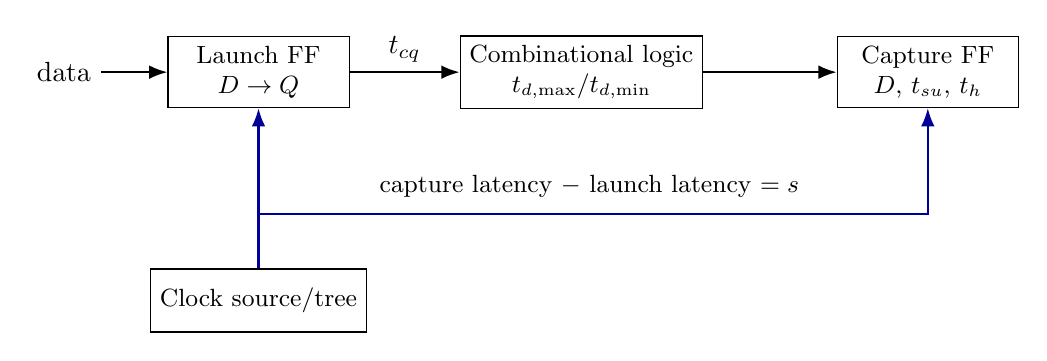
\begin{tikzpicture}[x=1cm,y=1cm]
  \node[block] (ff1) at (0,1.4) {Launch FF\\$D\rightarrow Q$};
  \node[block,minimum width=30mm] (comb) at (4.1,1.4) {Combinational logic\\$t_{d,\max}/t_{d,\min}$};
  \node[block] (ff2) at (8.5,1.4) {Capture FF\\$D$, $t_{su}$, $t_h$};
  \draw[datawire] (-2,1.4) node[left] {data} -- (ff1.west);
  \draw[datawire] (ff1.east) -- node[above] {$t_{cq}$} (comb.west);
  \draw[datawire] (comb.east) -- (ff2.west);
  \node[smallblock] (clk) at (0,-1.5) {Clock source/tree};
  \draw[clockwire] (clk.north) -- (0,-0.4) -- (0,0.65) -- (ff1.south);
  \draw[clockwire] (0,-0.4) -- (8.5,-0.4) -- (ff2.south);
  \node[signal] at (4.2,-0.05) {capture latency $-$ launch latency $=s$};
\end{tikzpicture}}

\or

\resizebox{\textwidth}{!}{%
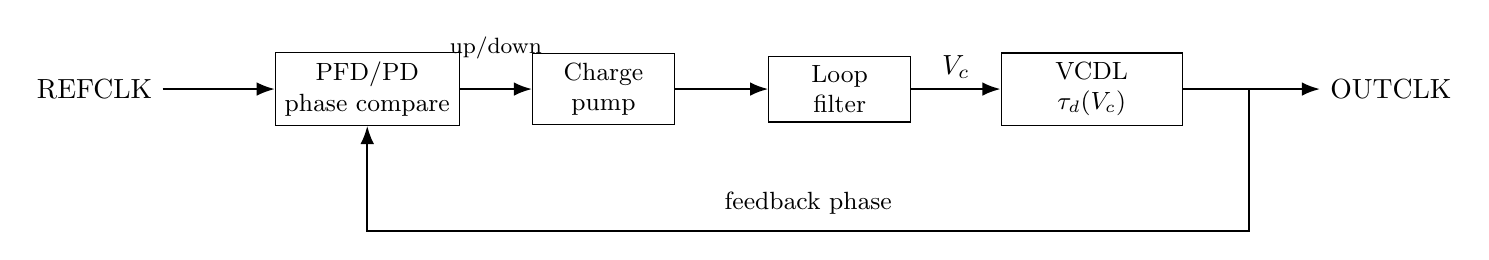
\begin{tikzpicture}[x=1cm,y=1cm]
  \node[smallblock] (pfd) at (0,0) {PFD/PD\\phase compare};
  \node[smallblock] (cp) at (3,0) {Charge\\pump};
  \node[smallblock] (lf) at (6,0) {Loop\\filter};
  \node[block] (vcdl) at (9.2,0) {VCDL\\$\tau_d(V_c)$};
  \draw[datawire] (-2.6,0) node[left] {REFCLK} -- (pfd.west);
  \draw[datawire] (pfd.east) -- node[above=2.5mm,font=\footnotesize] {up/down} (cp.west);
  \draw[datawire] (cp.east) -- (lf.west);
  \draw[datawire] (lf.east) -- node[above] {$V_c$} (vcdl.west);
  \draw[datawire] (vcdl.east) -- (12.1,0) node[right] {OUTCLK};
  \draw[datawire] (11.2,0) -- (11.2,-1.8) -- (0,-1.8) -- (pfd.south);
  \node[signal] at (5.6,-1.45) {feedback phase};
\end{tikzpicture}}

\or

\resizebox{\textwidth}{!}{%
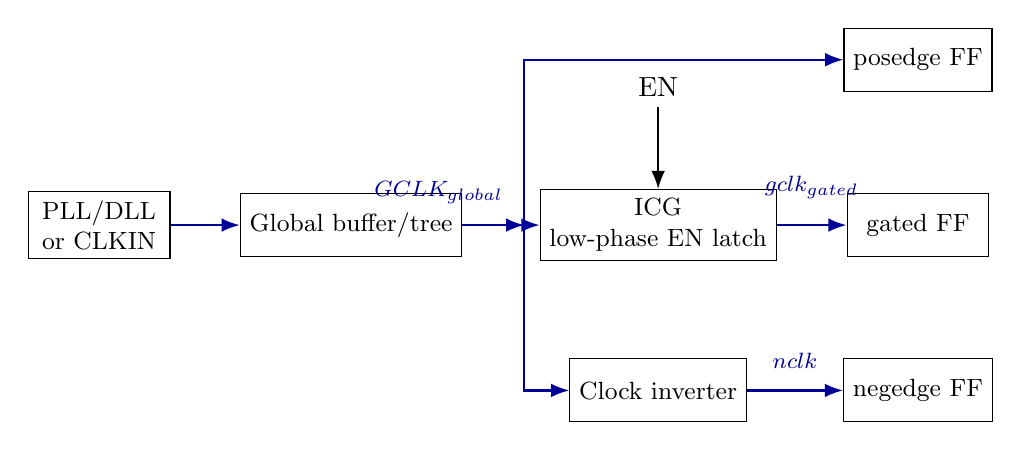
\begin{tikzpicture}[x=1cm,y=1cm]
  \node[smallblock] (src) at (0,0) {PLL/DLL\\or CLKIN};
  \node[smallblock] (tree) at (3.2,0) {Global buffer/tree};
  \draw[clockwire] (src.east) -- (tree.west);
  \draw[clockwire] (tree.east) -- (5.4,0)
    node[above left=2mm,font=\footnotesize] {$GCLK_{global}$};
  \node[smallblock] (ffp) at (10.4,2.1) {posedge FF};
  \draw[clockwire] (5.4,0) -- (5.4,2.1) -- (ffp.west);
  \node[smallblock] (icg) at (7.1,0) {ICG\\low-phase EN latch};
  \node[smallblock] (ffg) at (10.4,0) {gated FF};
  \draw[clockwire] (5.4,0) -- (icg.west);
  \draw[clockwire] (icg.east) -- node[above=2mm,font=\footnotesize] {$gclk_{gated}$} (ffg.west);
  \draw[datawire] (7.1,1.5) node[above] {EN} -- (icg.north);
  \node[smallblock] (inv) at (7.1,-2.1) {Clock inverter};
  \node[smallblock] (ffn) at (10.4,-2.1) {negedge FF};
  \draw[clockwire] (5.4,0) -- (5.4,-2.1) -- (inv.west);
  \draw[clockwire] (inv.east) -- node[above=1.5mm,font=\footnotesize] {$nclk$} (ffn.west);
\end{tikzpicture}}

\or

\resizebox{\textwidth}{!}{%
\begin{tikzpicture}[x=1cm,y=1cm]
  \node[smallblock] (da) at (0,1.6) {Driver A};
  \node[smallblock] (ra) at (3,1.6) {$R_A$};
  \node[smallblock] (rb) at (3,-1.8) {$R_B$};
  \node[smallblock] (db) at (0,-1.8) {Driver B};
  \draw[datawire] (da.east)--(ra.west);
  \draw (ra.east)--(8.5,1.6) node[right] {Receiver A};
  \draw[datawire] (db.east)--(rb.west);
  \draw (rb.east)--(8.5,-1.8) node[right] {Receiver B};
  \draw (5.5,1.6)--(5.5,0.75);
  \draw (5.15,0.75)--(5.85,0.75);
  \draw (5.15,0.52)--(5.85,0.52);
  \draw (5.5,0.52)--(5.5,-0.15) node[below] {$C_A$ to ground};
  \draw (5.5,-1.8)--(5.5,-2.55);
  \draw (5.15,-2.55)--(5.85,-2.55);
  \draw (5.15,-2.78)--(5.85,-2.78);
  \draw (5.5,-2.78)--(5.5,-3.25) node[below] {$C_B$ to ground};
  \draw (7,1.6)--(7,0.25);
  \draw (6.65,0.25)--(7.35,0.25);
  \draw (6.65,0.02)--(7.35,0.02);
  \draw (7,0.02)--(7,-1.8);
  \node at (7.7,-0.65) {$C_c$};
  \fill (5.5,1.6) circle (1.3pt);
  \fill (5.5,-1.8) circle (1.3pt);
  \fill (7,1.6) circle (1.3pt);
  \fill (7,-1.8) circle (1.3pt);
\end{tikzpicture}}

\fi
\end{document}
